 \documentclass[12pt,english]{article}
\usepackage[utf8]{inputenc}
\markright{Pearse et al.\hfill Assessing the Effects Imputation on ED Values\hfill}
\usepackage{geometry}
\geometry{verbose,letterpaper,tmargin=2.54cm,bmargin=2.54cm,lmargin=2.54cm,rmargin=2.54cm}
%\geometry{verbose,letterpaper,tmargin=.1cm,bmargin=.1cm,lmargin=.1cm,rmargin=.1cm}
\usepackage{graphicx}
\DeclareGraphicsExtensions{.pdf,.png,.jpg}
\usepackage{amssymb,amsmath}
\usepackage{epstopdf}
\usepackage{tocbibind}
\usepackage[toc,page]{appendix}
\usepackage{supertabular}
\DeclareGraphicsRule{.tif}{png}{.png}{`convert #1 `dirname #1`/`basename #1 .tif`.png}
\usepackage{url}
\usepackage{subcaption}
\usepackage{caption}
\usepackage[super]{nth}
\usepackage{lineno} \linenumbers
\usepackage[doublespacing]{setspace}
\usepackage[parfill]{parskip}
\setlength{\parindent}{0pt}
\usepackage[citestyle=authoryear,bibstyle=authoryear,sorting=nyt,maxcitenames=2,maxbibnames=10,minbibnames=6,doi=false,url=false,isbn=false,firstinits=true,uniquename=false,uniquelist=false]{biblatex}
\bibliography{edge_sims}
\renewbibmacro*{name:andothers}{% Based on name:andothers from biblatex.def
  \ifboolexpr{
    test {\ifnumequal{\value{listcount}}{\value{liststop}}}
    and
    test \ifmorenames
  }
    {\ifnumgreater{\value{liststop}}{1}
       {\finalandcomma}
       {}%
     \andothersdelim\bibstring[]{andothers}}
    {}}
\renewcommand*{\finalnamedelim}{%
  \ifnumgreater{\value{liststop}}{2}{\finalandcomma}{}%
  \addspace\&\space}
\renewbibmacro{in:}{}
\AtEveryBibitem{%
  \clearfield{day}%
  \clearfield{month}%
  \clearfield{endday}%
  \clearfield{endmonth}%
}
\DeclareFieldFormat[article]{citetitle}{#1}
\DeclareFieldFormat[article]{title}{#1}
\DeclareFieldFormat[article]{pages}{#1}
\DeclareNameAlias{sortname}{last-first}

\usepackage{changes}
\setdeletedmarkup{\textcolor{red}{\sout{#1}}}

\begin{document}
\setlength{\parindent}{0pt}
\section*{Title page}

\textbf{Article title}: Assessing the Effects Imputation on ED Values

\textbf{Running head}: Assessing the Effects Imputation on ED Values

\textbf{Authors:} K.\ Bodie Weedop$^{1}$, William D.\ Pearse$^{1}$\

$^1$ Department of Biology \& Ecology Center, Utah State University,
5305 Old Main Hill, Logan UT, 84322

$^*$To whom correspondence should be addressed:
\url{will.pearse@usu.edu}

\textbf{Word-count}: 5680 (abstract, main text, acknowledgments, and
  references)

\clearpage
\section*{Abstract}


\textbf{Keywords}: 

\clearpage
\section*{Introduction}

% A real blinder of a 

% Arg, Bodie, I'm sorry: I habitually re-format text while I'm typing,
% which I realise has likely just messed up track changes for you in
% these first two paragraph. Sorry, I'll try and stop doing it going
% forward...

Evidence from the fossil record and present-day studies argue we are
in the midst of, or entering, a sixth mass extinction
\autocite{Barnosky2011, Ceballos2015}, such that more species than
ever are declining and/or in danger of extinction across a range of
environments \autocite{Wake2008,Thomas2004}. Habitat destruction
\autocite{Brooks2002}, invasive species \autocite{Molnar2008}, climate
change \autocite{Pounds2006}, and disease \autocite{Lips2006} are some
of the leading causes of species declines globally. Conservation
biologists seek to reverse these declines and their detrimental
effects on species populations, but in reality they have limited
resources with which to do so. This challenge, termed the ``Noah's Ark
problem'' \autocite{Weitzman1998}, has driven conservation biologists
to prioritize, or triage, the resource allocation
\autocite{Bottrill2008}.
% Again, be precise: "confront this issue" --> what issue?...

Conservation triage, like all sound decision-making, requires some
metric that quantifies the \replaced{[put something here that's a bit
  more precise. Importance != endangerment != urgency, so pick
  something and go with that]}{importance and degree of endangerment
  urgency for a set of species}. By using such a metric, researchers
are able to avoid biasing the allocation of time and resources for
conservation, and can make their conservation goals more explicit.
One such triage strategies which has been widely used is the EDGE
metric\autocite[Evolutionary Distinction and Globally
Endangered;][]{Isaac2007}. This method prioritizes species according
to two metrics: Evolutionary Distinctiveness (ED) and Global
Endangerment (GE).
% Global endangerment isn't actually a metric... 
ED measures relative contributions to phylogenetic
diversity made by each species within a particular
clade\autocite{Isaac2007}, assigning each branch length equally to all
its subtending species.
% ...something like this...
GE values are assessed by
assigning numerical values to each of the World Conservation Union
(IUCN) Red List Categories.
The precise mapping of numerical values onto each category varies, and
can affect the relative rankings of EDGE species \autocite{Mooers2008}.
\replaced{I'm not sure you need this sentence. You could, if you wish,
  say something more about the different kinds of rankings, or perhaps
  how there are different ways of doing the ED bit (e.g., the Redding
  paper, which is similar but slightly different---Equal Splits)}
{As species become increasingly
threatened and are placed into more concerning categories
(\emph{e.g.}, from Vulnerable to Endangered), the GE numerical value
increases.} Thus a species' EDGE score is intended to equally reflect a species'
evolutionary distinctiveness and conservation status \autocite[but
see][for discussion on this]{Pearse2015}.

The EDGE approach was never intended to be a purely academic metric,
and is now the basis of the global EDGE of Existence Program
(\url{http://www.edgeofexistence.org/}). While EDGE was originally used to prioritize global mammals, it has subsequently been applied to a number of species groups.

There are now EDGE lists of amphibians \autocite{Isaac2012}, birds \autocite{Jetz2014}, corals
\autocite{Curnick2015}, and sharks \autocite{Stein2018}. A 
number of similar metrics  have been developed,
each prioritizing and emphasizing subtly different things, such as the
expected contribution of each species to overall phylogenetic
diversity \autocite[HEDGE;][]{Steel2007}, our uncertainty over a
species' future \autocite[EDAM;][]{Pearse2015}, and the
complementarity of a set of species \autocite{Faith2008,Jensen2016}.
Thus the development of EDGE-like metrics has matched progress with other fields of conservation biology, where the
likelihood of success in conservation \autocite{Wilson2007, Mcbride2007},
relative cost of certain interventions\autocite{Naidoo2006}, and complementarity
of interventions\autocite{Pressey1993, Myers2000} have also been considered
. % You might want to re-structuer what I've done above in the light
  % of this sentence; I'll leave that up to you
Critically, EDGE has formed the basis of a successful program that quantitatively
prioritizes conservation, providing actionable insights into how to focus
conservation effort in the face of uncertainty about species' attributes. EDGE's success proves that phylogenetic conservation prioritization metrics can be used by
conservation biologists and policy makers, and that they are popular with the public. Nonetheless, almost every application
of an EDGE-like approach has had to deal with the uncertainty presented by missing species data.

The IUCN has a well-established protocol for how to deal with
data-deficient species: they are to be treated as if they were of
Endangered species to ensure consistency \autocite[check this
Bodie][]{Rodrigues2006}. The problem, however, is arguably more
complex for species whose phylogenetic position is unknown.
Species of conservation concern are almost by definition rare, and so
we frequently lack sufficient DNA (or even morphological) data to
place them with certainty on a phylogeny. In the face of such essentially unavoidable uncertainty, 
conservation biologists have worked hard to overcome data limitations.
In most empirical EDGE lists, taxonomic information, rather
than sequence data alone, is used to locate species in the tree of life 
\autocite{Isaac2007, Isaac2012, Jetz2014, Curnick2015, Stein2018}.% Cite the tetrapod paper by Rikki here?
By using taxonomic information alone, researchers are able to produce fully
resolved phylogenies using model-based imputation \autocite{Kuhn2011}.% Maybe cite PASTIS here - the Thomas paper
Yet, to our knowledge, there has yet to be a systematic study of the effect of such imputation on species' EDGE scores, unlike in other aspects of comparative biology \autocite{Rabosky2014}.
Indeed, there is no clear guidance as to the size of the effect of
ignoring missing species on remaining species during prioritization,
or the magnitude of error phylogenetic imputation introduces. % Make this a little neater if you wish; I use the word "error twice!"
As the desire to use ED and
phylogenies for conservation triage grows, the importance of such tests and a
consensus on how to resolve cases of phylogenetic uncertainty becomes more
urgent.
% I've trimmed this paragraph a little, just because I don't think we
% want to "give away the story" and I also think it's important not to
% piss people off in the intro. Let's stick to describing the data:
% that way we can't be controversial.

Here we quantify the effect of missing species on EDGE rankings and assess
whether imputing species is a defensible method for dealing with species
missing phylogenetic data. We do so by simulating the removal of species from simulated trees in two ways: at random and
in a phylogenetically biased manner. By doing so, we hope to provide
two reasonably realistic case-studies of how species might be expected to be missing
from the tree of life. We also assess the extent to which imputed species' EDGE rankings
correlate with their true values. To do this, we
simulate phylogenies, choose clades at random to remove, and then impute the structure
of these clades, all under the same model of diversification. In so doing
, we hope to provide clear guidance as to the applicability of phylogenetic imputation
as a solution for species missing phylogenetic data
.
From our results, we argue that species' ED values are remarkably
robust to the loss of species, and that phylogenetic imputation is not
reliable at reconstructing the true ranking of species.
% Don't reference results in the introduction - give a throw-away,
% like this, if you're going to give the results.

\section*{Methods}
% This is good: here is what it needs, though. Make a conceptual
% diagram showing (1) correlating the ED scores before and after
% removal from the tree, and (2) the imputation of species ED scores
% in clades. You can then write at the bottom of each of the figures
% what this will help us answers ("are missing species a problem for
% the ED scores of other species?"; "can imputation fill in for
% missing species")

Here we use a simulation approach to test the effect of removing and imputing
species on a phylogeny on species' ED (Evolutionary Distinctiveness) scores
. Since empirical studies do not (to our knowledge) impute GE (Global
Endangerment) scores for species, instead relying on the IUCN's proposal to treat Data Deficient species as XXX (e.g., shark paper?), we focus solely on phylogenetic imputation
. EDGE is
the product of both ED and GE, thus perfectly accurate GE values could still lead to a  biased EDGE score
if the ED scores were imperfectly calculated.

All simulations and analyses were performed using R \autocite[version
3.4.0;][]{R2017}, and we performed 100 replicate simulations of each parameter combination
. All trees (both starting and imputed) were
simulated under a pure-birth Yule model using the \texttt{sim.bdtree} function
in the \texttt{geiger} R package \autocite[wrong citation; there's a newer one with Matt Pennell as the first author][]{Harmon2007}.
% What parameter value for lambda?
This particular model was
chosen because it is the simplest model possible: speciation rates are constant across the entire tree of life and there is no extinction.
We acknowledge that it is possible that more complex and/or
biologically realistic models of diversification could improve the
performance of imputation. However, we suggest that imputation under a
simple model that is identical to that used to simulate the data is
a low benchmark for a method to surpass.
We used \texttt{ed.calc} in the R package \texttt{caper}
to calculate ED values \autocite{Orme2013}.

\subsection*{The impact of missing species on EDGE scores}
Our first set of simulations assesses the impact of random and
phylogenetically-biased loss of species from a phylogeny on ED scores.
Both sets of simulations were carried out
using phylogenies of different sizes (number of taxa: 64, 128, 256, ..., 2048,
4096), removing constant fractions of tips from the tree (0\%, 1\%, 2\%, ...,
19\%, ..., 99\%).
To simulate randomly missing species, we used the \texttt{sample}
function in R to select the relevant percentage of species (rounded to
the nearest whole number?) without replacement. 
Thus this randomization did not incorporate phylogenetic structure.
To remove species in a phylogenetically biased manner, we used
\textcite{Felsenstein2005}'s threshold model. First, we simulated a
trait under a constant rate Brownian-motion model ($\sigma^2$=0.5,
starting root value = 1).
% Using what function/package?
Species were then removed from the tree if their simulated trait was
in the upper quantile of whatever fraction of species were to be
dropped. For example, if
10\% of species were to be dropped, species within the upper \nth{10} quantile of
character trait values were removed from the tree.

We calculated species' ED values before removal of species from the
tree and afterwards. We then correlated the ED scores of the species
left in the tree with their original ED values, to measure the effect
of species' removal on ED scores. To see if phylogenetic structure
could explain variation in the effect of removal, we also recorded,
before species were removed from the tree, \added{XXX list all the
  things you recorded here and give citations for them, taken from the
  functions' help files if you're uncertain.} 
If missing species
have no effect upon ED values, we expect a high, positive coefficient of
correlation between the remaining species' ED scores before and after
the other species were removed from the tree.

% Do you need to repeat this with different sigma values?
% Hmmm, what?? -Bodie
% WDP: line 246 above you mention \sigma. That's what I mean. Perhaps
%      this doesn't matter; I've added some text to account for this.

\subsection*{The impact of phylogenetic imputation on EDGE scores}
We tested the impact of imputing missing species onto clades of various sizes
(3, 4, 5, ..., 30, 31, 32 species) from phylogenies of different sizes
(64, 128, 256, 512, and 1024 species). We first randomly selected
a clade to be removed from the original tree, simulated a new phylogeny of
the same size under the same pure-birth model used to generate the phylogeny, and placed the newly
simulated clade back where the original clade was removed. Thus we imputed
each clade under the model used to generate it: in an empirical study this model
would, itself, have to be inferred but we do not address this
additional source of error here.
\added{In cases where a phylogeny was simulated without a clade of the
  required size (XXX cases), that particular simulation was aborted
  and we moved on to the next simulation. In cases where a clade could
  not be simulated after XXX attempts that was sufficiently young to
  be inserted into the phylogeny (XXX cases), that simulation was also
  aborted and the next simulation.}

To assess whether clades, once imputed, had similar ED scores, we
correlated the imputed ED scores against true ED scores.
We also calculated the sum of the absolute change in ranked ED for
each species, which is particularly relevant for EDGE-listing as it is
often the top 100, 200, etc., species on which conservation actions
are targeted.
We statistically modeled both these metrics as a function of the
number of total species and number of species within an imputed clade,
since we might expect larger clades and/or larger phylogenies to be
imputed more erroneously.

\section*{Results}
Under both random and phylogenetically-patterned loss, species' ED
scores are less accurate as more species are removed from the tree
(Table 1; Fig. \ref{randomVsClustered}). \added{What is the
  correlation when 10\% and 20\% of species are missing at random?}
Phylogenetically biased loss of species affects ED scores more
strongly (Table 1; Fig.\ \ref{randomVsClustered}), but the effect is
comparable to random loss (XXX values as you gave for random loss).

\begin{figure}[!ht]
  \center
  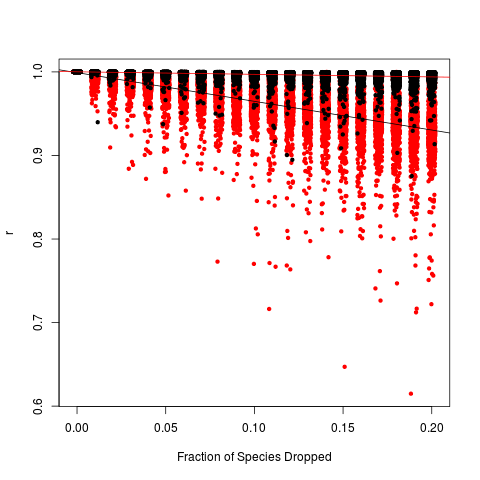
\includegraphics[width=.5\textwidth]{randomVsCluster.png}
  \caption{\textbf{R-values plotted against the fraction of species dropped at
  random versus clustered manner.} The color of data points denote whether
  species were dropped at random (orange; n = 100) or in clustered manner
  (grey; n = 100). The regression lines are demonstrating the relationship when
  species are dropped at random (red) and in a clustered manner (clustered). The
  correlations represent a comparison of the ED values (before and after
  species are dropped) of species which remain on the on the phylogeny after
  other species are dropped. 
  }
  \label{randomVsClustered}
\end{figure}

\begin{table}[ht]
  \centering
  \begin{tabular}{rrrrr}
    \hline
      & Estimate & Std. Error & t value & Pr($>$$|$t$|$) \\
      \hline
      (Intercept) & 1.0315 & 0.0013 & 821.39 & $<$0.0001 \\
      Fraction of Species Dropped & -0.4696 & 0.0020 & -233.16 & $<$0.0001 \\
      Random Treatment & 0.0630 & 0.0018 & 35.47 & $<$0.0001 \\
      Number of Species Overall & 0.0000 & 0.0000 & 7.89 & $<$0.0001 \\
      Fraction of Species Dropped:Random Treatment & -0.2774 & 0.0028 & -97.45 & $<$0.0001 \\
      Random Treatment:Number of Species Overall & 0.0000 & 0.0000 & -4.38 & $<$0.0001 \\
      \hline
    \hline
  \end{tabular}
\caption*{\textbf{Table 1: ANCOVA model summary describing the effect of
dropping species on remaining species ED Values.} The fraction of species
dropped significantly affects the the remaining ED values. Dropping the
fraction both at random and in clustered manner both have negative effects on
the remaining ED values ($F_{139696, 5}$ = 40350, $R^{2}$ = 0.5908,
p$<$0.0001).}
\end{table}

We find no support for a correlation between the imputed and true ED values for
species within imputed clades (Fig. \ref{imputationTrend}, Table 2). We found
that measures of the true phylogeny such as phylogenetic diversity (PD), estimated rate of diversification $\hat{\lambda}$,
Colless' Index, skew, and kurtosis
% skew and kurtosis of what?
do not provide any indication that imputation
would negatively affect ED values (Appendix A). We do find evidence that, when
imputing larger clades, the variation in the correlation is lesser
(Fig. \ref{quantReg}), but the correlation between true and imputed ED values appear
to converge on zero correlation (Table 3).
Imputed rankings of species within clades are also altered
under imputation (Fig. \ref{rankingError}; Table 4); \added{quote some exemplar numbers to give an impression of the degree of problem}.
This ranking error increases with the size of the imputed clade and
phylogeny (Table 4), and can affect ranking error within the top 100,
250, etc. species (Appendix B).

\begin{figure}[!ht]
  \center
  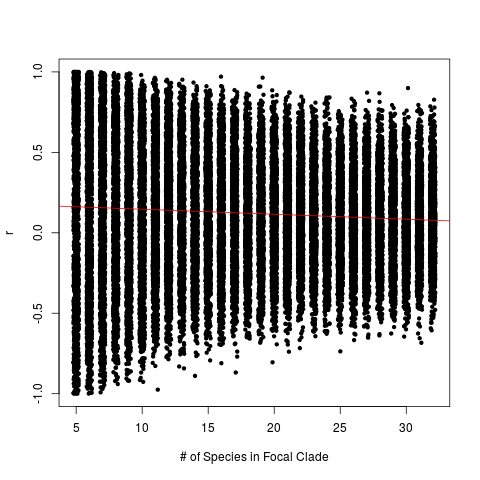
\includegraphics[width=.5\textwidth]{edModel.png}
  \caption{\textbf{R-values plotted against the number of species at focal
  clade.} Each data point denotes a correlative comparison between ED values
  within the focal clades where imputation has occurred. The regression line
  (red) and trend even closer to zero demonstrates the decrease in informative
  value of the imputed ED values. This is reinforced by the visual narrowing of
  r-values around zero.}
  \label{imputationTrend}
\end{figure}

\begin{table}[ht] 
\centering
\begin{tabular}{rrrrr}
  \hline
  & Estimate & Std. Error & t value & Pr($>$$|$t$|$) \\
   \hline
   (Intercept) & 0.1691 & 0.0500 & 3.38 & 0.0007 \\
   Size of Focal Clade & -0.0029 & 0.0002 & -14.15 & 0.0000 \\
   Size of Phylogeny & -0.0001 & 0.0001 & -1.01 & 0.3128 \\
   PD & 0.0001 & 0.0001 & 0.97 & 0.3339 \\
   Lambda & 0.0051 & 0.0492 & 0.10 & 0.9179 \\
   Colless' Index & 0.0020 & 0.0021 & 0.96 & 0.3388 \\
   Skew & 0.0039 & 0.0083 & 0.47 & 0.6409 \\
   Kurtosis & -0.0005 & 0.0008 & -0.64 & 0.5247 \\
   \hline
   \hline
\end{tabular}
\caption*{\textbf{Table 2: Effect of Clade Size on Imputed ED Values.} The
intercept describes that the correlation between the true and imputed values
begins quite low. As the clade size increases, this correlation only tends
toward zero. The total number of species in the full phylogeny along with
measures of the true phylogenetic diversity, lambda, Colless' Index, skew, and
kurtosis show no significant effect. ($F_{47992, 7}$ = 29.38, $R^{2}$ = 0.005,
p$<$0.0001).}
\end{table}

\begin{figure}[!ht]
  \center
  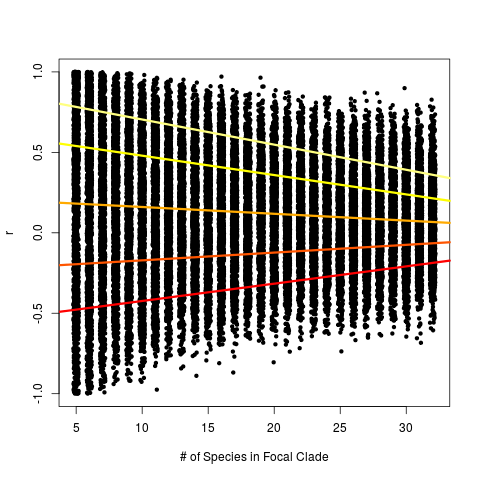
\includegraphics[width=.5\textwidth]{quantModel.png}
  \caption{\textbf{Quantile regression of r-values against size of imputed
  clades.} Each data point denotes a correlative comparison between ED values
  within the focal clades where imputation has occurred. Each regression line
  (top to bottom) represent quantile regressions from highest to lowest,
  respectively. Each of the regression lines demonstrate a convergence of the
  variation in r-values around zero.}
  \label{quantReg}
\end{figure}

\begin{table}[ht]
  \centering
  \begin{tabular}{rrrrrr}
    \hline
  & \tau = 0.10 & \tau = 0.25 & \tau = 0.50 & \tau = 0.75 & \tau = 0.90 \\
    \hline
  (Intercept) & -0.54 & -0.23 & 0.20 & 0.60 & 0.86 \\
    Size of Focal Clade & 0.01 & 0.01 & -0.00 & -0.01 & -0.02 \\
    \hline
    \hline
  \end{tabular}
  \caption*{\textbf{Table 3: Quantile Regression of Clade Size and Total Species
  on Ranking Error.} Quantile regression model demonstrating the effect of clade
  size on the correlation between true and imputed ED values. The quantile
  regression estimates demonstrate statistical significance that as imputed
  clade size increases, variation in coefficient of correlation (r) between ED
  values center around zero (all p-values are $<$0.0001).}
\end{table}


\begin{figure}[!ht]
  \center
  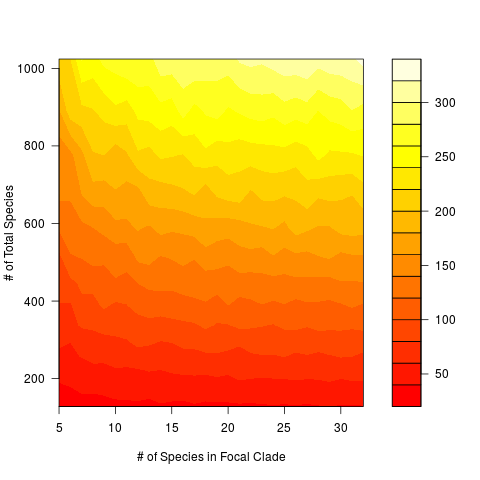
\includegraphics[width=.5\textwidth]{rankingError.png}
  \caption{\textbf{Mean ranking error of species within the focal clade.} The 
  gradient on the right demonstrates average number of positions within the 
  full ranking that focal clade species shifted from their true rank.
  While controlling for the size of the full phylogeny and focal clade, species 
  within the focal clade were, on average, ranked far from the true rank. }
  \label{rankingError}
\end{figure}

\begin{table}[ht]
  \centering
  \begin{tabular}{rrrrr}
    \hline
   & Estimate & Std. Error & t value & Pr($>$$|$t$|$) \\
    \hline
  (Intercept) & -1.6344 & 0.0332 & -49.29 & 0.0001 \\
    Size of Focal Clade & 0.0900 & 0.0010 & 91.22 & 0.0001 \\
    Size of Phylogeny & 0.5179 & 0.0013 & 383.99 & 0.0001 \\
     \hline
     \hline
  \end{tabular}
  \caption*{\textbf{Table 4: Effect of Clade Size and Total Species on Ranking
  Error.} Model demonstrating the relationship between focal clade species
  ranking error and the size of imputed clade and overall phylogeny. Square-root
  transformations have been applied to both ranking error and size of phylogeny.
  Significant increases ranking error are seen when increasing sizes of both the
  imputed clade and phylogeny ($F_{47997, 2}$ = 77890, $R^{2}$ = 0.7644,
  p$<$0.0001).}
  \end{table}

\clearpage
\section*{Discussion}
Phylogenetic conservation prioritization is an emerging tool providing a much
needed, objective measure for conservation decision-making and policy. However,
phylogenetic uncertainty is a major obstacle for EDGE and similar metrics
\autocite{Collen2015}. Uncertainty in phylogenies could mean that species in
desperate need of conservation effort are overlooked. In order to address such
uncertainty, we aim to determine how removing missing species from a phylogeny
affects ED values for the remaining species and demonstrate how imputation
affects ED values of species where imputation is performed. Our results
demonstrate that missing a proportion of overall species both at random and in a
phylogenetic-biased manner have different yet significant affects on remaining
ED values throughout the tree and imputation does not recover the ED value or ED
rank of an imputed species.

Our results are derived solely from simulations under a simple model of
diversification---the Yule model. We do acknowledge that, in the real world,
lineages evolve in more complex ways than are captured by such a simple model.
While we do not have empirical data, imputing species under this model should be
much easier given the simplicity. We have not been given any implication through
this investigation that a more complex model would produce any different result.
Therefore, we suggest that our results generalize from the simplest case to more
complicated cases which might be seen in empirical data. However, our results
demonstrate that even under a simple model imputing species lead to a
misrepresentation of true ED values. 

Normally, imputation and artificially, fully resolved clades are achieved by
generating a pseudo-posterior distribution of numerous trees, using a
birth-death model of evolution, for clades where there are unsampled species
using a polytomy resolver \autocite{Kuhn2011}. However, our results demonstrate
that there is uncertainty in that pseudo-distribution of trees being used to set
priorities (Fig. \ref{imputationTrend}).

\subsection*{Uncertainty in imputed species}
Missing species and poor phylogenetic resolution have been identified as causes
of uncertainty when calculating ED \autocite{Isaac2007}. Prior to our
investigation, we could not find any assessment of how missing species might
affect ED values of species which are not missing. In previous research,
incomplete phylogenies were shown to produce nearly the same result as the
later, more complete trees \autocite{Curnick2015}. While demonstrating EDGE
scores derived in the face of phylogenetic uncertainty still perform quite well
in setting accurate priorities, they did not explicitly test the effect which
missing species, nor imputing missing species, has on ED values. Our results
support the finding that missing species do affect ED scores but the effect is
relatively insignificant compared to percentages of species missing (Table 1). 

We realize that we have provided just two ways in which species could be missing
from a phylogeny and there are more that could occur. Missing species could be
biased by some phylogenetic pattern other than Brownian motion evolution.
Nevertheless, our investigation shows that missing species cause ED values of
species remaining in the phylogeny to deviate from the true value. This effect
should be considered when debating whether under other, more complex models of
evolution a different effect might be seen. There could be cases where species
could be missing from the phylogeny with the result that an entire clade is
unsampled. This would be a case of species radiating in situ and have persisted
in one, restricted area. A situation such as this is seen with corals in the
Indian Ocean region \autocite{Arrigoni2012}.

In the past, we have included missing species into the EDGE framework using
different methods. Collen et al. assigned the mean ED score of presumed
congeneric species to the missing species \citeyear{Collen2011}. More
frequently, missing species and poorly resolved clades have been dealt with by
imputing the missing species and assigning all the species of the resolved clade
the mean ED value obtained from all possible or numerous resolutions of the
clade \autocite{Isaac2007; Isaac2012}. This method has been adapted by others
and applied where there were large percentages (~30\% or 3,330 species) missing
\autocite{Jetz2014}. 

While imputation does include missing species, relying upon taxonomic information
and constraints under some estimated model of evolution could become is
subjective. Kuhn et al. \citeyear{2011} suggests that when using their polytomy
resolver, the application of the of the resolver will be biased by the model of
evolution estimated. More recent research confirms, that when under the prior of
a birth-death model, imputation methods consistently bias evolutionary rates and
estimates of phylogenetic signal used in downstream analyses
\autocite{Rabosky2014}. 

When considering the analysis of ED, our results show that imputation does not
recover true ED values nor ED rank of missing species (Fig. \ref{imputationTrend};
 Fig. \ref{rankingError}). As the size of the imputed clade increases, ED values of imputed
species do not correlate with their true values (Table 2). Even though we are
including missing species into calculating ED, we are not obtaining accurate
information about those species. While being uninformative, these ED values
would also lead to mispriortizing species based on our results. In the event
that a clade of 25 species in a phylogeny of 850 species, our results show those
imputed species would be, on average, 250 ranks from their true rank (Fig.
\ref{imputationTrend}; Table 4). Analyzing the performance of imputation of a
clade less than five species was not performed because we can't report a
correlation reliably with so little data \autocite{Crawley2012}. Even still, we
cannot see how the trend in our results would suddenly change such that, when
imputing only one species, it improves.  
% * Invoke Arne's 'the clade should have an average ED' argument to
%   support this. In smaller clades (i.e., two species, and you don't
%   know where that species goes) then you should just be sampling from
%   the prior. That prior is exponential, and so there's absolutely no
%   reason to suppose it will do any better than what we have
%   already. This is a more complicated argument, so have a bash at it
%   and then we can talk.

% I would like to go over this a bit more -Bodie

\subsection*{Guidelines for the use of imputation}
We suggest there is a straightforward synthesis of these results that should be
useful in applied conservation biology. Both random and
phylogenetically-patterned loss of species affect ED values throughout the tree.
However, we found that ED values of non-imputed species remain constant under
imputation. Therefore, imputation could be used to avoid missing species biasing
ED values of non-missing species. We have shown that imputing missing species
would not provide accurate ED values for missing species. However, it would
provide a method of avoiding the loss of species affecting ED values throughout
the remainder of the tree. Basing conservation priorities upon the ED values of
imputed species would lead to inaccurate prioritization. Nevertheless,
imputation may be useful to stop missing species from biasing species easily
placed on the phylogeny. 

Given these results, we now present guidelines for how missing species should be
dealt with and when imputation might be appropriate when calculating EDGE. Our
aim is to provide a rule of thumb for the use of imputation and how imputed
species should be handled. In the event of missing species, researchers should
be investigating the exact amount of species that are missing and consider
whether imputation is necessary. Our analyses show that even with a large
proportion of species missing, ED values of remaining species are highly
correlated. For some context, in our analysis we found that 30\% of species
missing at random or in a phylogenetic-biased manner from the phylogeny leads to
a correlation coefficient of 0.8 and 0.89, respectively. Therefore if species
are missing, we should verify that the amount of missing species does not exceed
a percentage which we have found to provide poor ED values for remaining
species. While below an acceptable percentage of missing species, EDGE should be
carried out without attempting to impute the missing species. However, if a
larger proportion of species are missing, imputation may be used but with some
caution. ED values for species easily placed on the phylogeny are relatively
unaffected and can be trusted when setting conservation priorities.
Nevertheless, ED values and ranks of species which have been imputed should
either be ignored or used cautiously within EDGE. Our results demonstrate that
an individual species within an imputed clade of 25 species on a phylogeny of
1024 species is, on average, ranking $\pm$ ~318 positions from its true rank (Fig. 
\ref{rankingError}).
While imputation does not affect ED values of known species, includes missing
species in the phylogeny, it does not help understand the true ranking of an
imputed species. By following these guidelines we avoid biasing species which
are easily placed on the phylogeny and confounding the rankings for the sake of
including missing species.

\section*{Acknowledgments}

\clearpage
\printbibliography

\clearpage
\appendix
\section*{A. Effect of Measures of the True, Full Phylogenies}

\begin{figure}[!ht]
  \center
  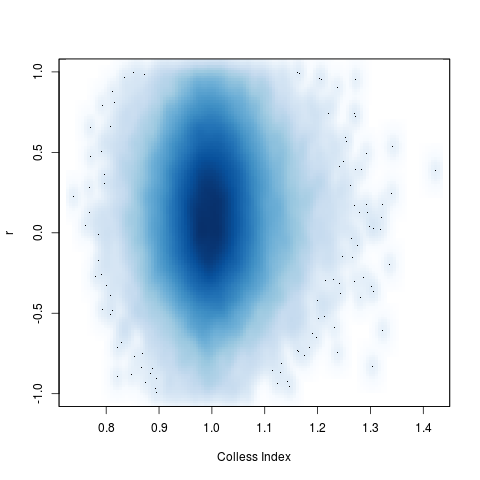
\includegraphics[width=.5\textwidth]{trueColless.png}
  \caption{\textbf{Effect of the True Colless Index of FullPhylogeny.}}
\end{figure}

\begin{figure}[!ht]
  \center
  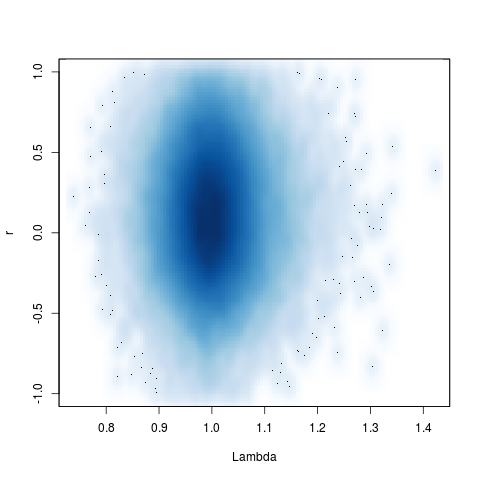
\includegraphics[width=.5\textwidth]{trueLambda.png}
  \caption{\textbf{Effect of the True Lambda of Full Phylogeny.}}
\end{figure}

\begin{figure}[!ht]
  \center
  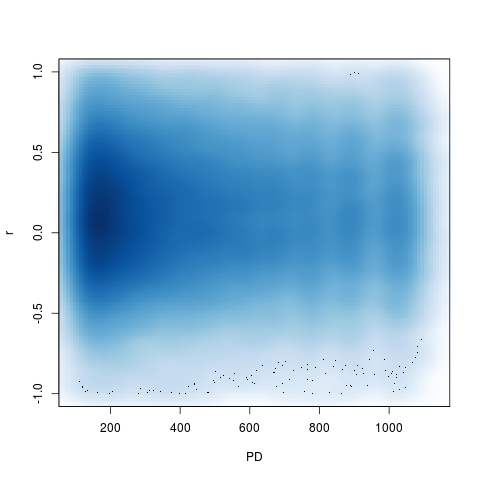
\includegraphics[width=.5\textwidth]{PD.png}
  \caption{\textbf{Effect of True PD of Full Phylogeny.}}
\end{figure}

\begin{figure}[!ht]
  \center
  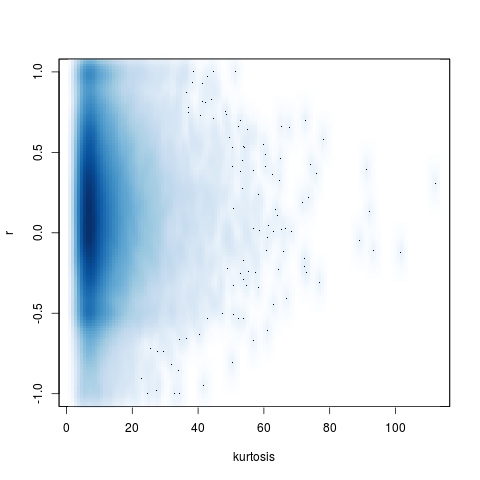
\includegraphics[width=.5\textwidth]{originalKurtosis.png}
  \caption{\textbf{Effect of the True Kurtosis of Full Phylogeny.}}
\end{figure}

\begin{figure}[!ht]
  \center
  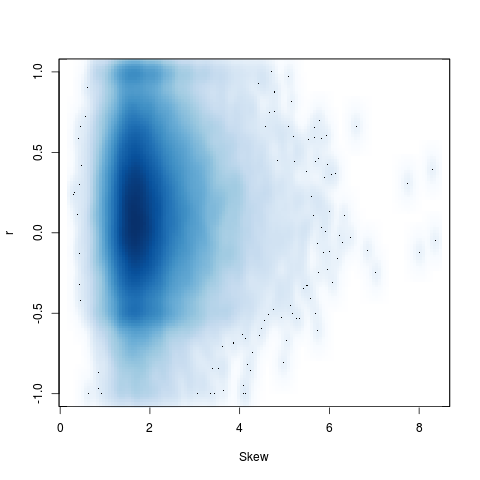
\includegraphics[width=.5\textwidth]{originalSkew.png}
  \caption{\textbf{Effect of the True Skew of Full Phylogeny.}}
\end{figure}

\clearpage
\clearpage
\section*{B. Error Rate in Top Rankings}

\begin{figure}[!ht]
  \center
  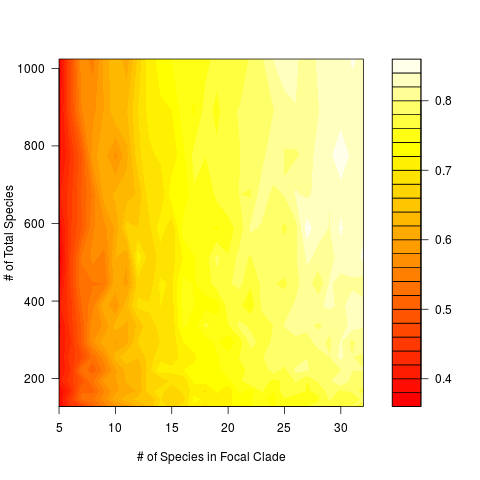
\includegraphics[width=.5\textwidth]{errorRate50.png}
  \caption{\textbf{Mean error rate in the ranking of top 50 species.}}
\end{figure}

\begin{figure}[!ht]
  \center
  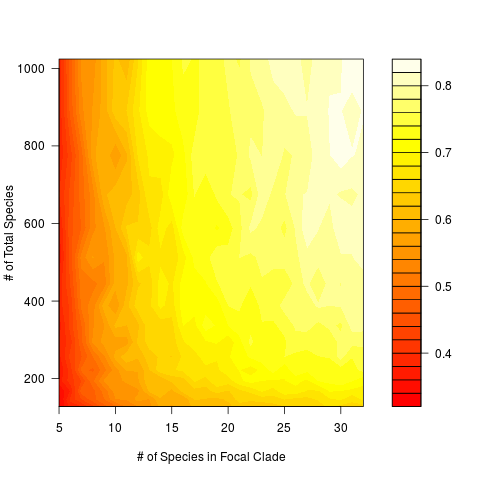
\includegraphics[width=.5\textwidth]{errorRate100.png}
  \caption{\textbf{Mean error rate in the ranking of top 100 species.} }
\end{figure}

\begin{figure}[!ht]
  \center
  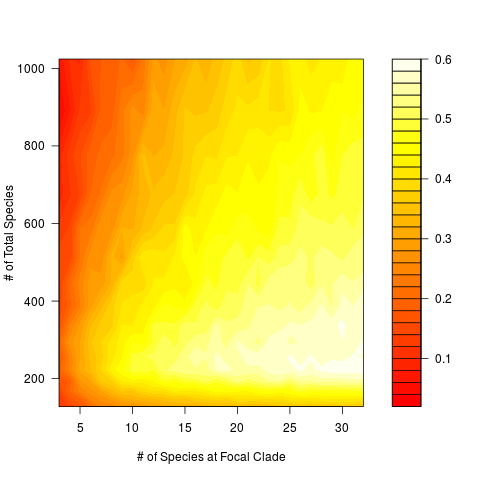
\includegraphics[width=.5\textwidth]{errorRate200.png}
  \caption{\textbf{Mean error rate in the ranking of top 200 species.} }
\end{figure}

\begin{figure}[!ht]
  \center
  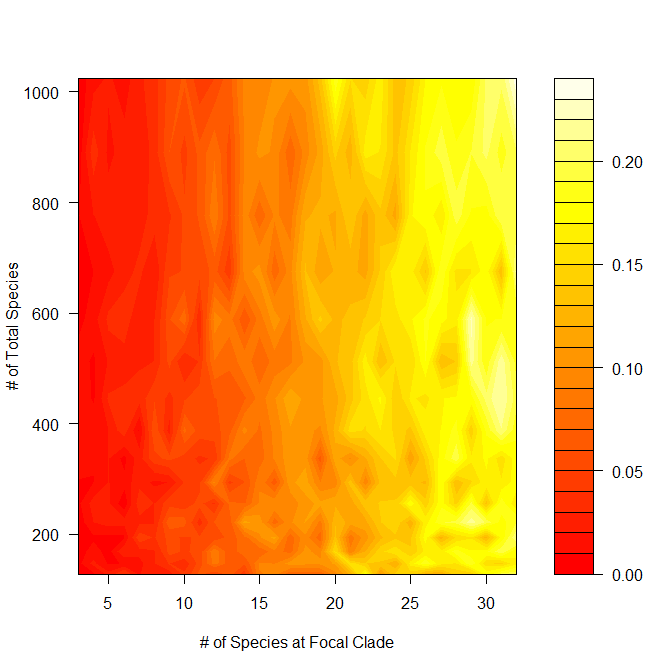
\includegraphics[width=.5\textwidth]{errorRate5pct.png}
  \caption{\textbf{Mean error rate in the ranking of top 5\% of species.} }
\end{figure}

\begin{figure}[!ht]
  \center
  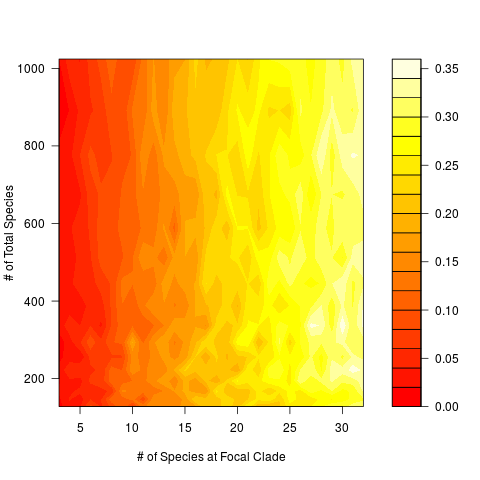
\includegraphics[width=.5\textwidth]{errorRate10pct.png}
  \caption{\textbf{Mean error rate in the ranking of top 10\% of species.} }
\end{figure}

\begin{figure}[!ht]
  \center
  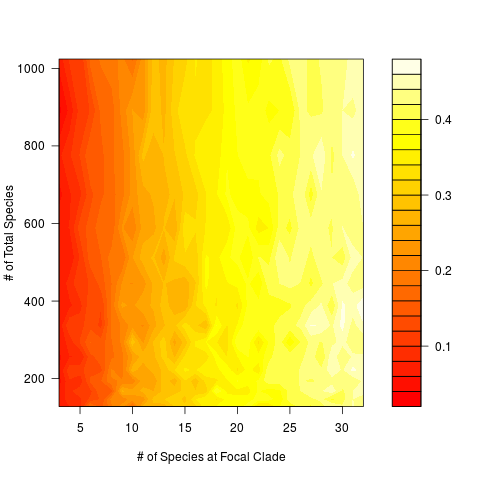
\includegraphics[width=.5\textwidth]{errorRate20pct.png}
  \caption{\textbf{Mean error rate in the ranking of top 20\% of species.}}
\end{figure}

\end{document}
%%% Local Variables:
%%% mode: latex
%%% TeX-master: t
%%% End:
